\section{Massively Learning Activities I - Initial Deployment} \label{section: MLA}
The System Development Life-cycle (SDLC) is a project management model that defines different stages that are necessary to bring a project from conception to deployment and later maintenance. The SDLC model consists of several phases: planning, requirement gathering, design, implementation, testing \& integration, and operations \& maintenance. It provides a systematic approach to system development that helps ensure that system is built efficiently with minimal risk.

Massively Learning Activities will follow a similar variation to the SDLC project management model where each SDLC stage will correspond to a subsection in this chapter.

\begin{figure}[H]
    \centering
    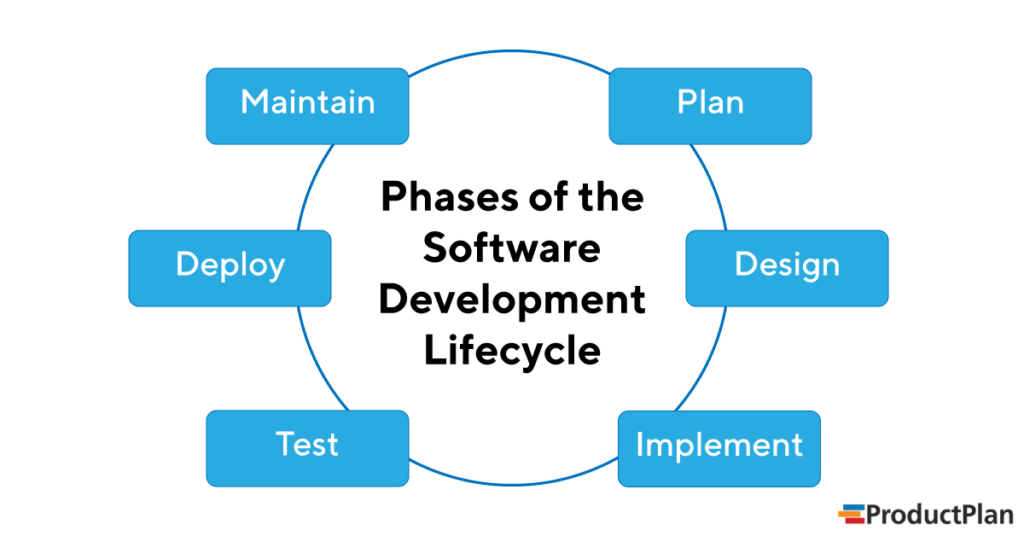
\includegraphics[scale = 0.25]{images/SDLC_Framework.png}
    \caption{System Developerment Life-Cycle \textcolor{red}{(STOLEN EXAMPLE)} }
    \label{SDLC}
\end{figure} 

%----------------------------------------------------------------------------------%

\subsection{Planning I} 

TASI has been contracted by CNMI to create an infrastructure that will allow for data analytics on Protected Health Information (PHI). To achieve this, TASI will provide a Platform as a Service (PaaS) solution, by hosting SAS services on on-premises hardware, configured for multi-tenancy.

Tenants will provide the data, which will be submitted through an ETL pipeline for data migration, cleaning, and processing. Once the data has been processed, tenants may perform data analytics using advanced algorithms in SAS programming language.

Due to SAS being a time sensitive project, the initial deployment will have SAS suites and VMs installed on existing hardware, with plans to migrate the infrastructure to newly acquired hardware in the future.

MLA I will expect 4 tenants:
\begin{enumerate}
    \item Commonwealth of the Northern Mariana Islands (CNMI)
    \item All-Payer Claims Database (APCD)
    \item Centers for Medicare \& Medicaid Services (CMA)
    \item Med-Quest
\end{enumerate}

\subsection{Requirement of Analysis I}

The Requirement Analysis phase is a crucial component in developing a robust SAS infrastructure using the SDLC framework. This phase involves gathering and analyzing the specific requirements for the project, including pre-installation checklists and EEC sizing requirements. In this phase, ongoing project management tasks will be performed, such as preparing a project plan and assigning appropriate resources. 

Furthermore, as part of this phase, SAS will send a Pre-Install Requirements Document to the client for completion, and both parties will ensure environmental readiness for installation by reviewing the completed document. 

Additionally, SAS will send a billable work hours log for verification based on the project plan. This subsection will provide a detailed overview of the pre-installation checklist and EEC sizing requirements necessary for a successful implementation of the SAS infrastructure.

\newpage 

\subsubsection{Multi-Tenancy Configuration Plan: VM Location}
\label{Multi-Tenancy Configuration Plan}

\begin{figure}[H]
\begin{center}
    \renewcommand{\arraystretch}{1.5}
    \begin{tabular}{|>{\raggedright\arraybackslash}l 
                    |>{\raggedright\arraybackslash}m{6cm} 
                    |>{\raggedright\arraybackslash}l 
                    |>{\raggedright\arraybackslash}l 
                    |>{\raggedright\arraybackslash}l 
                    |}
    \hline
    \rowcolor[HTML]{196fb4}\centering\textcolor{white}{\large Server Name} 
                            & \centering\textcolor{white}{\large Function} 
                            & \centering\textcolor{white}{\large Type} 
                            & \centering\textcolor{white}{\large Site} 
                            & \centering\textcolor{white}{\large Physical Server} 
                            \tabularnewline 
    \hline
    DC1	           & LDAP Host1                         & VM & ITS M01 & FX2Blade4 \\\hline
    DC2	           & LDAP Host2                         & VM & ITS M01 & FX2Blade1 \\\hline
    SAS 9.4 Server & SAS Infrastructure Server          & VM & ITS M01 & FX2Blade2 \\\hline
    SAS DMA	       & SAS Data Management Advanced       & VM & ITS M01 & NaN	\\\hline
    SAS Ansible	   & Ansible	                        & VM & ITS M01 & NaN	\\\hline
    SAS PRT	       & SAS Programming Run-Time	        & VM & ITS M01 & NaN	\\\hline
    SAS SL	       & SAS Service Layer	                & VM & ITS M01 & NaN	\\\hline
    Provider CC1   & Provider Primary CAS Controller    & VM & ITS M01 & NaN	\\\hline
    Provider CC1   & Provider Backup CAS Controller     & VM & ITS M01 & NaN	\\\hline
    R1 CC1	       & Research 1 CAS Controller 1	    & VM & ITS M01 & NaN	\\\hline
    R1 CC2	       & Research 1 CAS Controller 2	    & VM & ITS M01 & NaN	\\\hline
    R1 W1	       & Research 1 CAS Worker 1	        & VM & ITS M01 & NaN	\\\hline
    R1 W2	       & Research 1 CAS Worker 2	        & VM & ITS M01 & NaN	\\\hline
    R1 W3	       & Research 1 CAS Worker 3	        & VM & ITS M01 & NaN	\\\hline
    R2 CC1	       & Research 2 CAS Controller 1	    & VM & ITS M01 & NaN	\\\hline
    R2 CC2	       & Research 2 CAS Controller 2	    & VM & ITS M01 & NaN	\\\hline
    R3 W1	       & Research 3 CAS Worker 1	        & VM & ITS M01 & NaN	\\\hline
    R3 W2	       & Research 3 CAS Worker 2	        & VM & ITS M01 & NaN	\\\hline
    R3 W3	       & Research 3 CAS Worker 3	        & VM & ITS M01 & NaN	\\\hline
    R4 CC1	       & Research 4 Primary CAS Controller  & VM & ITS M01 & NaN	\\\hline
    R4 CC2	       & Research 4 Backup CAS Controller   & VM & ITS M01 & NaN	\\\hline
    R4 W1	       & Research 4 CAS Worker 1	        & VM & ITS M01 & NaN	\\\hline
    E1 CC1	       & Education 1 Primary CAS Controller & VM & ITS M01 & NaN	\\\hline
    E1 CC2	       & Education 1 Backup CAS Controller  & VM & ITS M01 & NaN	\\\hline
    E1 W1	       & Education 1 CAS Worker 1	        & VM & ITS M01 & NaN	\\\hline
    E2 CC1	       & Education 2 Primary CAS Controller & VM & ITS M01 & NaN	\\\hline
    E2 CC2	       & Education 2 Backup CAS Controller  & VM & ITS M01 & NaN	\\\hline
    E2 W1	       & Education 2 CAS Worker 1	        & VM & ITS M01 & NaN	\\\hline
    E3 CC1	       & Education 3 Primary CAS Controller & VM & ITS M01 & NaN	\\\hline
    E3 CC2	       & Education 3 Backup CAS Controller  & VM & ITS M01 & NaN	\\\hline
    E3 W1	       & Education 3 CAS Worker 1	        & VM & ITS M01 & NaN	\\\hline
    E4 CC1	       & Education 4 Primary CAS Controller & VM & ITS M01 & NaN	\\\hline
    E4 CC2	       & Education 4 Backup CAS Controller  & VM & ITS M01 & NaN	\\\hline
    E4 W1	       & Education 4 CAS Worker 1	        & VM & ITS M01 & NaN	\\\hline
    
    \end{tabular}
\end{center}
\caption{Physical and logical locations of VMs related to SAS technologies.}
\label{MTP-1}
\end{figure}

\subsubsection{Multi-Tenancy Configuration Plan: Resource Allocation}

\begin{figure}[H]
\begin{center}
    \renewcommand{\arraystretch}{1.5}
    \begin{tabular}{|>{\raggedright\arraybackslash}l 
                    |>{\raggedright\arraybackslash}l
                    |>{\raggedright\arraybackslash}l 
                    |>{\raggedright\arraybackslash}m{2cm}
                    |>{\raggedright\arraybackslash}l 
                    |>{\raggedright\arraybackslash}m{2cm} 
                    |>{\raggedright\arraybackslash}m{1.5cm} 
                    |}
    \hline
    \rowcolor[HTML]{196fb4}\centering\textcolor{white}{\large Server Name} 
                            & \centering\textcolor{white}{\large Tenant} 
                            & \centering\textcolor{white}{\large OS} 
                            & \centering\textcolor{white}{\large Memory (GB)} 
                            & \centering\textcolor{white}{\large vCPU}
                            & \centering\textcolor{white}{\large Min Sys Storage}
                            & \centering\textcolor{white}{\large Storage (GB)}
                            \tabularnewline 
    \hline
    DC1	           & NaN      & RHEL 8 & 12 & 4 & NaN & 50  \\\hline
    DC2	           & NaN      & RHEL 8 & 12 & 4 & NaN & 50  \\\hline
    SAS 9.4 Server & NaN      & RHEL 8 & 32 & 8 & NaN & NaN \\\hline
    SAS DMA	       & NaN      & RHEL 8 & 32 & 8 & NaN & NaN \\\hline
    SAS Ansible	   & NaN	  & RHEL 8 & 16 & 2 & NaN & NaN \\\hline
    SAS PRT	       & NaN	  & RHEL 8 & 64 & 6 & NaN & NaN \\\hline
    SAS SL	       & NaN	  & RHEL 8 & 32 & 2 & NaN & NaN \\\hline
    Provider CC1   & Provider & RHEL 8 &  8 & 2 & NaN & NaN \\\hline
    Provider CC1   & Provider & RHEL 8 &  8 & 2 & NaN & NaN \\\hline
    R1 CC1	       & Tenant 1 & RHEL 8 & 16 & 2 & NaN & NaN \\\hline
    R1 CC2	       & Tenant 1 & RHEL 8 & 16 & 2 & NaN & NaN \\\hline
    R1 W1	       & Tenant 1 & RHEL 8 & 16 & 2 & NaN & NaN \\\hline
    R1 W2	       & Tenant 1 & RHEL 8 & 16 & 2 & NaN & NaN \\\hline
    R1 W3	       & Tenant 1 & RHEL 8 & 16 & 2 & NaN & NaN \\\hline
    R2 CC1	       & Tenant 2 & RHEL 8 & 16 & 2 & NaN & NaN \\\hline
    R2 CC2	       & Tenant 2 & RHEL 8 & 16 & 2 & NaN & NaN \\\hline
    R3 W1	       & Tenant 2 & RHEL 8 & 16 & 2 & NaN & NaN \\\hline
    R3 W2	       & Tenant 2 & RHEL 8 & 16 & 2 & NaN & NaN \\\hline
    R3 W3	       & Tenant 2 & RHEL 8 & 16 & 2 & NaN & NaN \\\hline
    R4 CC1	       & Tenant 3 & RHEL 8 &  8 & 1 & NaN & NaN \\\hline
    R4 CC2	       & Tenant 3 & RHEL 8 &  8 & 1 & NaN & NaN \\\hline
    R4 W1	       & Tenant 3 & RHEL 8 &  8 & 1 & NaN & NaN \\\hline
    E1 CC1	       & Tenant 4 & RHEL 8 &  8 & 1 & NaN & NaN \\\hline
    E1 CC2	       & Tenant 4 & RHEL 8 &  8 & 1 & NaN & NaN \\\hline
    E1 W1	       & Tenant 4 & RHEL 8 &  8 & 1 & NaN & NaN \\\hline
    E2 CC1	       & Tenant 5 & RHEL 8 &  8 & 1 & NaN & NaN \\\hline
    E2 CC2	       & Tenant 5 & RHEL 8 &  8 & 1 & NaN & NaN \\\hline
    E2 W1	       & Tenant 5 & RHEL 8 &  8 & 1 & NaN & NaN \\\hline
    E3 CC1	       & Tenant 6 & RHEL 8 &  8 & 1 & NaN & NaN \\\hline
    E3 CC2	       & Tenant 6 & RHEL 8 &  8 & 1 & NaN & NaN \\\hline
    E3 W1	       & Tenant 6 & RHEL 8 &  8 & 1 & NaN & NaN \\\hline
    E4 CC1	       & Tenant 7 & RHEL 8 &  8 & 1 & NaN & NaN \\\hline
    E4 CC2	       & Tenant 7 & RHEL 8 &  8 & 1 & NaN & NaN \\\hline
    E4 W1	       & Tenant 7 & RHEL 8 &  8 & 1 & NaN & NaN \\\hline
    \end{tabular}
\end{center}
\caption{Resource requirements of VMs related to SAS technologies.}
\label{MTP-2}
\end{figure}

\subsubsection{EEC Sizing and Pre-Installation Checklist: File Path(s)}

The full EEC Sizing and Pre-Installation Checklist(s) documents can be found in:
\begin{itemize}
    \item PATH: $\backslash$ $\backslash$ .. 300 SAS Installation $\backslash$ 9.4 $\backslash$ EEC Sizing Results
    \item PATH: $\backslash$ $\backslash$ .. 300 SAS Installation $\backslash$ SAS Viya 3.5 $\backslash$ EEC Sizing Results
\end{itemize}

\subsubsection{EEC Sizing: SAS 9.4 (Summarized)}
This document provides sizing guidance for SAS Office Analytics/Data Management Advanced. The estimate provided assumes a typical implementation of SAS Office Analytics/Data Management Advanced and does not take into account any additional workloads or components that may be added. The estimate is based on a preferred hardware vendor with a given performance characteristic. It is recommended that the environment be closely monitored and scaled to support the required workloads to meet the business objectives.

\begin{enumerate}
    
    \item Hardware and Operation System Assumptions:
    \begin{figure}[H]
    \begin{center}
        \renewcommand{\arraystretch}{1.5}
        \begin{tabular}{|>{\raggedright\arraybackslash}m{8cm} 
                        |>{\raggedright\arraybackslash}l
                        |}
        \hline
        \rowcolor[HTML]{196fb4}\centering\textcolor{white}{\large Tier} 
                                & \centering\textcolor{white}{\large Cores$\backslash$RAM} 
                                \tabularnewline 
        \hline
        SAS Metadata Server & \vtop{\hbox{\strut 2 cores with 16GB RAM}
                                    \hbox{\strut (8 GB RAM per core minimum)}}\\\hline
        SAS Compute Server  & \vtop{\hbox{\strut 6 to 8 cores with 48 to 64GB RAM}
                                    \hbox{\strut (8 GB RAM per core minimum)}}\\\hline
        SAS Mid-Tier Server (Web-App Server) 
                            & \vtop{\hbox{\strut 2 cores with 24GB RAM}
                                    \hbox{\strut (24 GB RAM per server minimum)}}\\\hline
        \end{tabular}
    \end{center}
    \caption{Hardware estimate for SAS 9.4: SAS Data Management Advanced. }
    \label{DMA-HRDWR-EST}
    \end{figure}
    \begin{itemize}
        \item This response is based on Intel Xeon E5-2600v4 or Gold 6200/6300 series processor with a clock speed of at least 3.30 GHz running Windows Server 2019, 64 bit operating system.
        \item Core counts are guidelines only. These requirements may vary depending on the solutions installed or the number of users/sessions supported in accordance with Operating System Guidelines and SAS recommendations, page file space should be set to 1.5 to 2 times the amount of physical memory. The machines should be configured for maximum memory bandwidth; this will be dependent on the actual processors/machines selected.
    \end{itemize}
    \item SAS Environment and Configuration Assumptions:
    \begin{itemize}
        \item SAS tends to be I/O intensive. Consider the peak I/O throughput requirements of their system and work with their storage provider to ensure that the storage environment can provide the level of I/O required. A significant percentage of “performance problems” reported to SAS Technical Support can be directly attributed to insufficient levels of I/O throughput.
        \item Recommended I/O throughput rates for the SAS Data and SAS WORK file systems are as follows: for permanent SAS data files, your application throughput requirements may dictate a minimum I/O throughput rate of 100-150 MBs/sec per core, minimum, in the system. Reads and writes to the file system will occur during the ETL process. Chronic and heavy reads and writes are common for the SAS WORK file system. 
        \item Depending on the architecture and deployment, multiple compute tiers need access to a common data area. This may require the use of a centralized storage mechanism such as a Clustered File System (CFS).
    \end{itemize}
\end{enumerate}

This sizing estimate is based on a combination of guidelines provided by SAS R\&D, SAS Product Management, test data, and field experience. Our best practice is to provide the topology as developed by R\&D and try to provide as unified a presentation of the requirements as possible. When questions on deployment arises, the Sizing team defers to the account team.

\subsubsection{EEC Sizing: SAS Viya 3.5 (Summarized)}

This document provides sizing guidance for SAS Viya 3.5. The estimate is not a performance benchmark and does not provide any performance guarantee. The University of Hawai’i at Manoa is responsible for all costs associated with procuring any hardware. This estimate assumes that appropriate data management activities will happen outside of SAS In Memory, and resources for data management activities are not included in this exercise.

\begin{enumerate}
    
    \item Hardware and Resource Assumptions:
    \begin{figure}[H]
    \begin{center}
        \renewcommand{\arraystretch}{1.5}
        \begin{tabular}{|>{\raggedright\arraybackslash}l 
                        |>{\raggedright\arraybackslash}l
                        |}
        \hline
        \rowcolor[HTML]{196fb4}\centering\textcolor{white}{\large Resource Type} 
                                & \centering\textcolor{white}{\large Resource Count} 
                                \tabularnewline 
        \hline
        \# of Servers       & 5 (4 CAS Worker Nodes + 1 CAS Controller Node)   \\\hline
        CPU per server      & \vtop{\hbox{\strut CAS Worker Node: 2 x 8 cores Intel Xeon Gold 6234 processors (3.3 GHz)}
                                    \hbox{\strut CAS Controller Node: 1 x 8 cores Intel Xeon Gold 6234 processors (3.3 GHz)}}\\\hline
        Total cores         & 72 \\\hline
        Memory Clock Speed  & 2933 MHz \\\hline
        RAM per node        & \vtop{\hbox{\strut CAS Worker Node: 192 GB}
                                    \hbox{\strut CAS Controller Node: 92 GB}}\\\hline
        Operating System    & Red Hat Enterprise Linux \\\hline
        NIC                 & 10 GbE \\\hline
        SAS Version         & VIYA 3.5 \\\hline
        Local Disk per node & 2x 480 GB SSD \\\hline
        \end{tabular}
    \end{center}
    \caption{Hardware estimate for SAS Viya 3.5.}
    \label{VIYA-HRDWR-EST}
    \end{figure}
    \begin{itemize}
        \item This response is based on the Dell servers with Intel Xeon processors which assumes uncompressed data.
        \item Additional Recommendations: Server power settings need to be set to maximum, hyper-threading should be enabled for all production CPU's, storage drives should be SSD's instead of HDD's.
        \item Two additional servers are configured: 
        \begin{enumerate}
            \item SAS Programming Runtime Environment (SPRE) is the environment where SAS programs are executed. (4 cores, 96 GB RAM, 2 x 480 GB SSD). 
            \item Dev/Test is a sandbox server to test the development environment before production \\(16 cores, 192 GB RAM, 2 x 480 GB SSD).
        \end{enumerate}
    \end{itemize}
    
\end{enumerate}

This sizing estimate is based on a combination of guidelines provided by SAS R\&D, SAS Product Management and test data. Changes to the workload (in either number of sessions or data volumes), operating system, or preferred vendor or chipset may render this sizing as void. In the event of changes, the SAS Account Team should resubmit the questionnaire with the needed updates for reprocessing. 

\subsubsection{TASI's Infrastructure}
\label{TASI's Infrastructure Section Header}

TASI's infrastructure consists of (1) Dell PowerEdge FX2 Enclosure. The FX2 Enclosure is a 2U rack-based server located inside a server rack at the ITS data center (ITS M01). The FX2 Enclosure consists of (4) blades, which are modular server components that are installed within the FX2 Enclosure as seen Figure \ref{Current ENV}. Each blade is a self-contained server that contains one or more CPUs, memory, storage, and other components required to run applications and services as seen in Figure \ref{BLD-RSRC}.

Despite each blade in the FX2 Enclosure already being allocated to other TASI projects, the unused resources will be logically separated to establish a multi-tenant environment that can facilitate SAS technologies.

\begin{figure}[H]
    \centering
    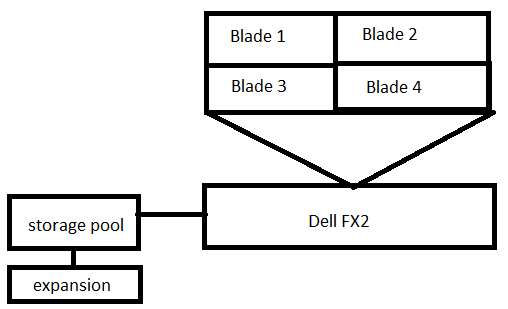
\includegraphics[scale = 0.70]{images/currentENV.png}
    \caption{TASI On-Premise Environment \textcolor{red}{(needs VISIO)} }
    \label{Current ENV}
\end{figure}

\begin{figure}[H]
\begin{center}
    \renewcommand{\arraystretch}{1.5}
    \begin{tabular}{|>{\raggedright\arraybackslash}l 
                    |>{\raggedright\arraybackslash}m{3cm}
                    |}
    \hline
    \rowcolor[HTML]{196fb4}\centering\textcolor{white}{\large Resource Type} 
                            & \centering\textcolor{white}{\large Resource Count (per Blade)} 
                            \tabularnewline 
    \hline
    CPU(s)              & 12 \\\hline
    Total cores         & XX \\\hline
    Memory              & 256GB RAM \\\hline
    Storage             & XX GB \\\hline
    Operating System    & ESXi 6.7 \\\hline
    \end{tabular}
\end{center}
\caption{Node count per Tenant}
\label{BLD-RSRC}
\end{figure}

\begin{figure}[H]
\begin{center}
    \renewcommand{\arraystretch}{1.5}
    \begin{tabular}{|>{\raggedright\arraybackslash}l 
                    |>{\raggedright\arraybackslash}l
                    |}
    \hline
    \rowcolor[HTML]{196fb4}\centering\textcolor{white}{\large Tenant} 
                            & \centering\textcolor{white}{\large Node Count} 
                            \tabularnewline 
    \hline
    Commonwealth of the Northern Mariana Islands (CNMI) & \vtop{\hbox{\strut (1) Primary CAS Controller }
                                                                \hbox{\strut (1) Backup CAS Controller}
                                                                \hbox{\strut (3) CAS Workers}}\\\hline
    All-Payer Claims Database (APCD)                    & \vtop{\hbox{\strut (1) Primary CAS Controller }
                                                                \hbox{\strut (1) Backup CAS Controller}
                                                                \hbox{\strut (3) CAS Workers}}\\\hline
    Centers for Medicare \& Medicaid Services (CMA)      & \vtop{\hbox{\strut (1) Primary CAS Controller }
                                                                \hbox{\strut (1) Backup CAS Controller}
                                                                \hbox{\strut (1) CAS Workers}}\\\hline
    Med-Quest                                           & \vtop{\hbox{\strut (1) Primary CAS Controller }
                                                                \hbox{\strut (1) Backup CAS Controller}
                                                                \hbox{\strut (1) CAS Workers}}\\\hline                                                            
    \end{tabular}
\end{center}
\caption{Resource count for a single Blade component.}
\label{TNTS-NDS}
\end{figure}

%----------------------------------------------------------------------------------%

\subsection{Design I}

The Design phase is a critical step in implementing a successful SAS infrastructure. During this phase, the technical specifications and architecture of the system are defined, and the appropriate hardware and software components are selected. This phase also includes creating a deployment plan, which outlines the steps for installing and configuring the system.

\subsubsection{Design Principles}

TASI will design a multi-tenant infrastructure that will accommodate all the VMs specified in the multi-tenancy configuration plan in Section \ref{Multi-Tenancy Configuration Plan}. The design should incorporate the architectural best practices of a \href{https://learn.microsoft.com/en-us/azure/well-architected/}{Well-Architected Framework}, which is a set design principles for running and designing workloads.

\begin{enumerate}
    \item Operational Excellence
    \begin{itemize}
        \item 
    \end{itemize}
    \item Reliability: A reliable application must be designed for failure by supporting high availability and disaster recovery principles. 
    \begin{itemize}
        \item CAS controller and CAS backup controller nodes must exist on separate hardware to support automated failover in the case of unexpected downtime. 
        \item TASI's on-premises infrastructure must have sufficient resources (e.g., compute, memory, storage) beyond the minimum requirement for supporting SAS technologies.
        \item All data that exists in volatile memory or storage should have regular backups. SAS loads data to be analyzed into non-volatile memory.
        \item All VMs should be scheduled for incremental backups and retention policies. 
    \end{itemize}
    \item Security: A secure application must be designed for confidentiality, integrity, and availability, whilst also adhering to new security standards such as authorization, encryption, monitoring, and auditing.
    \begin{itemize}
        \item Any data that TASI intends to store or process must comply with regulations and industry standards from HIPAA, UHM, RCUH, and other relevant compliance standards for protected health information.
        \item TASI must consider the principle of least privilege when designing an LDAP directory to support multi-tenancy.
        \item Data Governance: \textbf{\textcolor{red}{Fill me on May 24}}
        \item HIPPA compliance standards require data to be encrypted at-rest and in-transit. Data that is loaded in non-volatile memory for SAS, does not have to be encrypted. 
        \end{itemize}
    \item Performance Efficiency: An efficient application has the ability to use computing resources efficiently to meet system requirements, and maintains that efficiency as demand and technology changes.
    \begin{itemize}
        \item CAS worker nodes must be configured for MPP mode, where possible. 
        \item The SAS environment must be designed on infrastructure with ample resources beyond the minimum requirements to prevent potential bottlenecks as demand scales up.
        \item TASI must ensure that the servers have sufficient resources beyond the minimum requirements for VMs, to prevent potential bottlenecks when demand increases. 
        \item As the infrastructure grows, TASI must consider load balancing applications for user traffic across multiple servers. 
        \item To prepare for MLA II (VM Migration), TASI must ensure that their initial deployment is loosley coupled for scalability. This involves designing the infrastructure to be elastic, so it can handle sudden spikes in demand without compromising performance or availability.
    \end{itemize}
    \item Cost Optimization
    \begin{itemize}
        \item We will not have true cost optimization as we are using the CAPEX model. 
    \end{itemize}
\end{enumerate}

\subsubsection{IAM Design}

RCUH and UHTASI.

if uh then uh makes their own active directory. (check asana cause athena is working on that information with its

if tasi, we have to design our own LDAP system which is goin gto suck 

[user] -> [vpn] -> [connection is approved by LDAP]

\subsubsection{Multi-Tenancy}

The initial deployment of MLA will involve the installation of SAS 9.4 and SAS Viya 3.5 on existing infrastructure. The deployment configuration for each tenant will be tailored to meet their individual requirements. 

\begin{figure}[H]
    \centering
    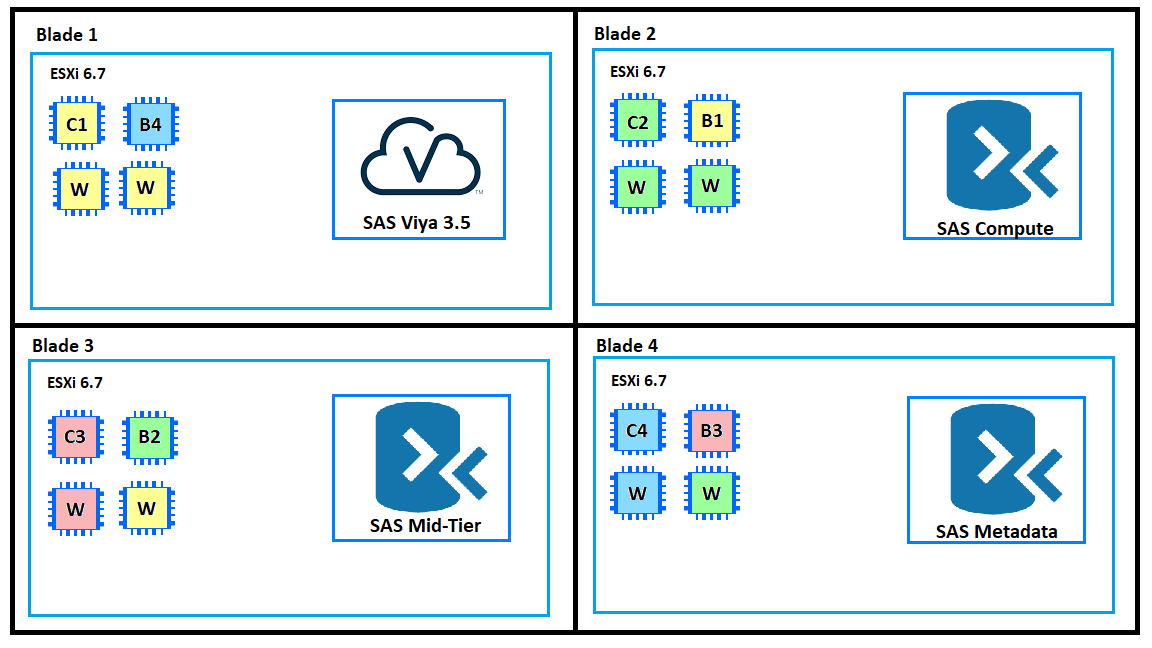
\includegraphics[scale = 0.52]{images/initial-deployment-diagram.png}
    \caption{Multi-Tenant Deployment \textcolor{red}{(needs VISIO)} }
    \label{Initial Multi-Tenant Deployment}
\end{figure} 

To maximize resource efficiency, CAS nodes will be evenly distributed across each blade, where a blade will consist of one controller, one backup controller, and two workers. The controller and backup controller, configured on the same system, will belong to separate tenants. The workers will also belong to separate tenants but each blade will have at least one related controller and worker per system. 

Subsequently, four additional VMs will be created to support the installation of SAS Viya 3.5 and SAS DMA. SAS Viya 3.5 will be installed as software on top of a RHEL 3.7X VM instance, in Blade 1. SAS DMA consists of three software components that will installed as software on top of Windows Server 2019 VM instances, in Blades' 2, 3, and 4. 

%----------------------------------------------------------------------------------%
\subsection{Implementation I}

April 18, 2023:
SAS 9.4 is installed first on TASI system. It is configured this way on blade 1. 

%----------------------------------------------------------------------------------%

\subsection{Testing \& Integration I}

%----------------------------------------------------------------------------------%

\subsection{Operations \& Maintenance I}